\input{../preamble.tex}

\lecturenumber{4}
\title{Process Creation}
\version{2.0.0}

\begin{document}
	\begin{frame}[plain, noframenumbering]
		\titlepage
	\end{frame}

	\begin{slide}
	
		\slidetitle{Running Processes On My Laptop}
		
		\centering
		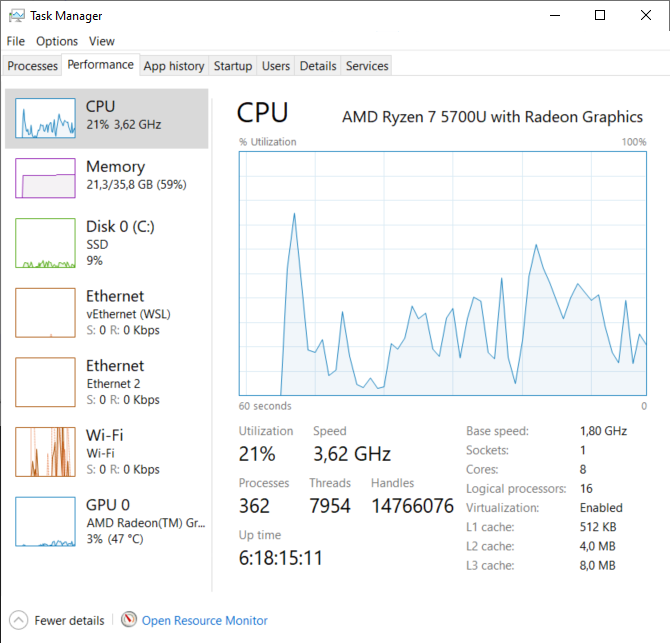
\includegraphics[width=60mm]{windows_num_process.png}
		
	\end{slide}
	
	\begin{slide}

		\slidetitle{Recall: A Process is an Instance of a Running Program}

		\centering
		\vspace{-8mm}
		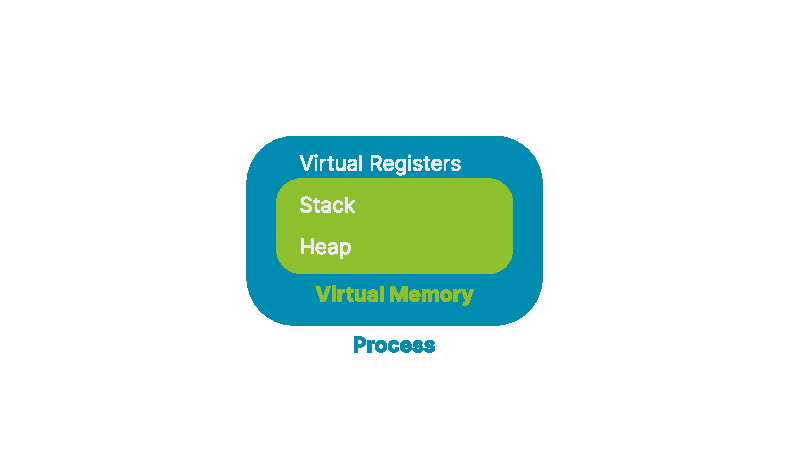
\includegraphics{../01-why-operating-systems/process-virtual-memory.eps}

	\end{slide}

	\begin{slide}

		\slidetitle{We Can Add More to a Process}

		\centering 
		\vspace{-8mm}
		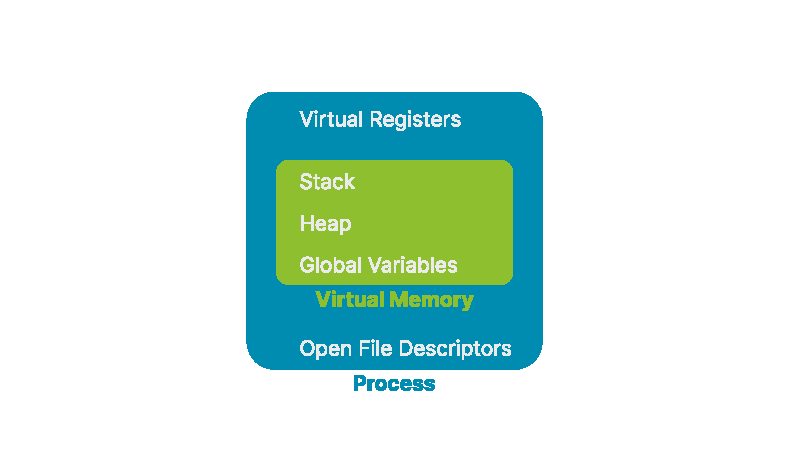
\includegraphics{process.eps}

	\end{slide}
	
	\begin{slide}

		\slidetitle{From The Kernel's Point of View}

		\centering 
		\vspace{-3mm}
		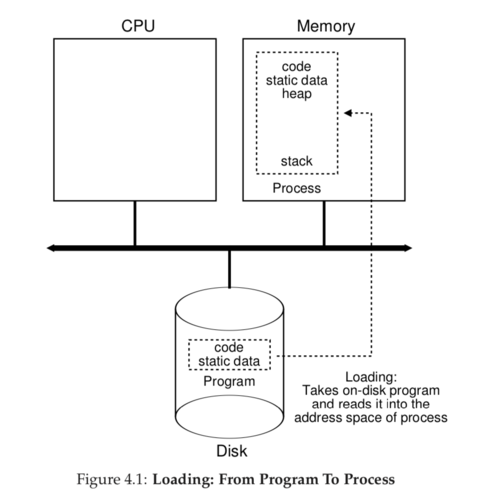
\includegraphics[width=60mm]{from_program_to_process.png}

	\end{slide}

	\begin{slide}

		\slidetitle{A Process Control Block (PCB) Contains All Information}

		Specifically, in Linux, this is the \texttt{\color{blue}
		task\_struct} you can browse on

		\href{https://github.com/torvalds/linux/blob/master/include/linux/sched.h\#L743}
			 {GitHub}
		\medskip

		It contains:
		\begin{itemize}
		  \item Process state
		  \item CPU registers
		  \item Scheduling information
		  \item Memory management information
		  \item I/O status information
		  \item Any other type of accounting information
		\end{itemize}
		\medskip

		Each process gets a unique process ID (pid) to keep track of it

	\end{slide}

\begin{slide}
	\slidetitle{Process State Diagram (You Could Rename Waiting to Ready)}

	\begin{tikzpicture}[
	  every initial by arrow/.style={rawarrow},
	  every state/.style={ellipse, minimum width=2.5cm, minimum height=1cm, font=\small},
	]
	  \node [state, initial] (created) {Created};
	  \node [state, right=of created] (waiting) {Waiting};
	  \node [state, above right=of waiting] (running) {Running};
	  \node [state, below right=of waiting] (blocked) {Blocked};
	  \node [state, accepting, below right=of running] (terminated) {Terminated};
	  \path [rawarrow] (created) edge (waiting)
				 (waiting) edge [bend left] (running)
				 (running) edge [bend left] (waiting)
				 (running) edge (blocked)
				 (blocked) edge (waiting)
				 (running) edge (terminated);
	\end{tikzpicture}
\end{slide}

\begin{slide}

	\slidetitle{You Can Read Process State Using the ``proc''
				Filesystem}

	There's a standard \texttt{/proc} directory (on Linux) that represents the kernel's
	state

	\leftspace{}These aren't real files, they just look like it!
	\medskip

	Every directory that's a number (process ID) in \texttt{/proc} represents a
	process
	\medskip

	There's a file called \texttt{status} that contains the state
	(used for Lab 1)

\end{slide}

\begin{slide}
	\slidetitle{We Could Create Processes from Scratch}

	We load the program into memory and create the process control block

	\leftspace{}(this is what Windows does)
	\bigskip

	Unix decomposes process creation into more flexible abstractions
\end{slide}

\begin{slide}

	\slidetitle{Instead of Creating a New Process, We Could Clone It}

	Pause the currently running process, and copy it's PCB into a new one

	\leftspace{}This will reuse all of the information from the process,
	including variables!
	\medskip


	Distinguish between the two processes with a parent and child relationship

	\leftspace{}They could both execute different parts of the program together
	\bigskip

	We could then allow either process to load a new program and setup a new PCB

\end{slide}

\begin{slide}

	\slidetitle{
	  \texttt{\bfseries fork} Creates a New Process, A Copy of the Current One
	}

	\mintinline{c}{int fork(void)} as the following API:
	\begin{itemize}
	  \item Returns the process ID of the newly created child process

			\leftspace{}-1: on failure

			\leftspace{}0: in the child process

			\leftspace{}>0: in the parent process
	\end{itemize}
	\medskip

	There are now 2 processes running

	\leftspace{}Note: they can access the same variables, but they're separate

	\leftspace{}\leftspace{}Operating system does ``copy on write'' to maximize sharing
\end{slide}
  
\begin{slide}

	\slidetitle{\texttt{\bfseries fork} Examples}
	
	\inputminted{c}{fork_example_1.c}
	
\end{slide}

 \begin{slide}

	\slidetitle{\texttt{\bfseries fork} Examples}
	
	\inputminted{c}{fork_example_1_2.c}
	
\end{slide}

\begin{slide}

	\slidetitle{\texttt{\bfseries fork} Examples}
	
	\inputminted{c}{fork_example_2.c}
	
\end{slide}

\begin{slide}

	\slidetitle{\texttt{\bfseries wait} delays execution}
	
	\texttt{wait} as the following API:
    \begin{itemize}
      \item \texttt{status}: Address to store the wait status of the process
      \item Returns the process ID of child process

            \leftspace{}-1: on failure

            \leftspace{}>0: the child with a change
    \end{itemize}
    \bigskip

    The wait status contains a bunch of information, including the exit code

    \leftspace{}Use \texttt{man wait} to find all the macros to query wait status

    \leftspace{}\leftspace{}You can use \texttt{waitpid} to wait on a specific child process

\end{slide}

\begin{slide}

	\slidetitle{\texttt{\bfseries wait} Example}
	
\begin{minted}{c}
int main() {
    int pid = getpid();
    fork();
    if (getpid() == pid){
        // wait(NULL);
        printf("Hello A\n");
    }
    else{
        printf("Hello B\n");
    }
    return 0;
}
\end{minted}
	
\end{slide}

  \begin{slide}

    \slidetitle{
      \texttt{\bfseries execve} Replaces the Process with Another Program, and
      Resets
    }

    \texttt{execve} has the following API:
    \begin{itemize}
      \item \texttt{pathname}: Full path of the program to load
      \item \texttt{argv}: Array of strings (array of characters), terminated by
             a null pointer

            \leftspace{}Represents arguments to the process
      \item \texttt{envp}: Same as \texttt{argv}

            \leftspace{}Represents the environment of the process
      \item Returns an error on failure, does not return if successful
    \end{itemize}
  \end{slide}

  \begin{slide}

    \slidetitle{
      \texttt{\bfseries execve-example.c} Turns the Process into
      \texttt{\bfseries ls}
    }

    \begin{minted}{c}
int main(int argc, char *argv[]) {
  printf("I'm going to become another process\n");
  char *exec_argv[] = {"ls", NULL};
  char *exec_envp[] = {NULL};
  int exec_return = execve("/usr/bin/ls", exec_argv, exec_envp);
  if (exec_return == -1) {
    exec_return = errno;
    perror("execve failed");
    return exec_return;
  }
  printf("If execve worked, this will never print\n");
  return 0;
}
    \end{minted}
  \end{slide}

  \begin{slide}
    \slidetitle{The Operating System Creates Processes}

    The operating system has to:
    \begin{itemize}
      \item Maintain process control blocks, including state
      \item Create new processes
      \item Load a program, and re-initialize a process with context
    \end{itemize}

  \end{slide}

\end{document}
